\section*{Appendix}

\subsection*{Diagramme}
In diesem Abschnitt werden manche der verwendeten Abbildungen in gr��erer Version aufgef�hrt.

%Kapitel2
\begin{figure}[H]
    \centering
    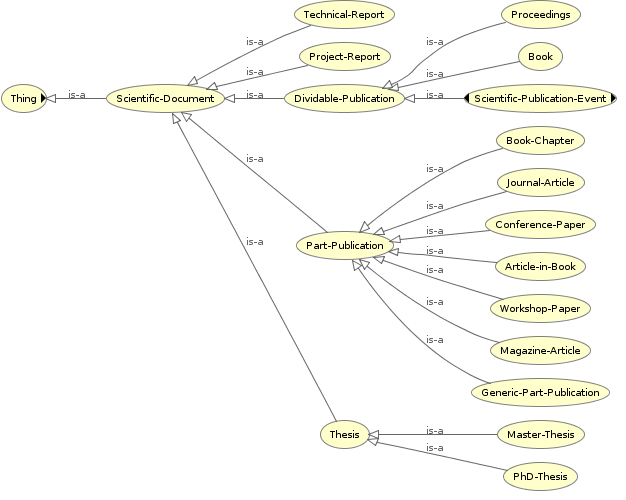
\includegraphics[angle=90,scale=0.65]{../deps/ontology_of_science_scientificdoc_owlviz.png}
    \caption{Ontology of Science. Die Klasse \textit{Scientific Document}}
    \label{fig:scientificdociBig}
\end{figure}

%Kapitel 3
\begin{figure}[H]
        \centering
        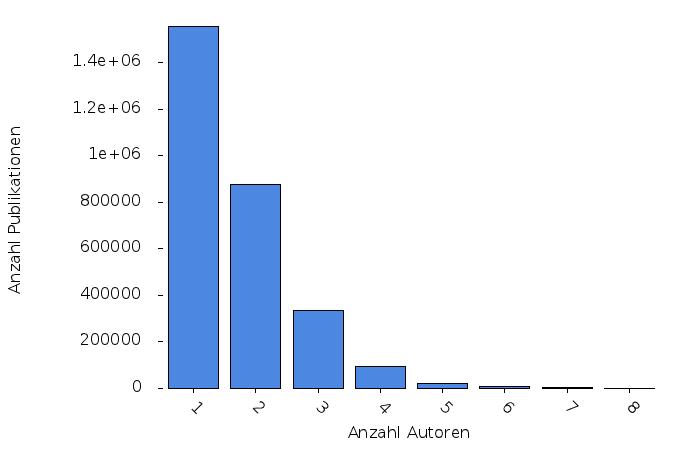
\includegraphics[scale=0.5]{../data/statistics/authorFreq.png}
        \caption{Autorenverteilung}
        \label{fig:authorFreqBig}
\end{figure}

\begin{figure}[H]
        \centering
        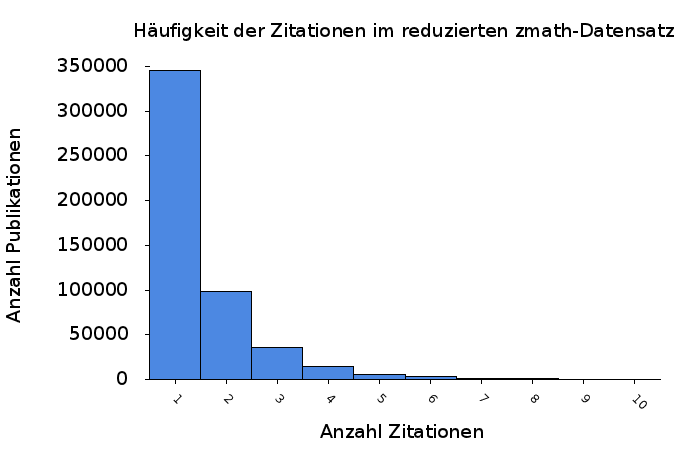
\includegraphics[scale=.5]{../data/statistics/citationFreq.png}
        \caption{Zitationsverteilung}
        \label{fig:citationFreqBig}
\end{figure}

\begin{figure}[H]
        \centering
        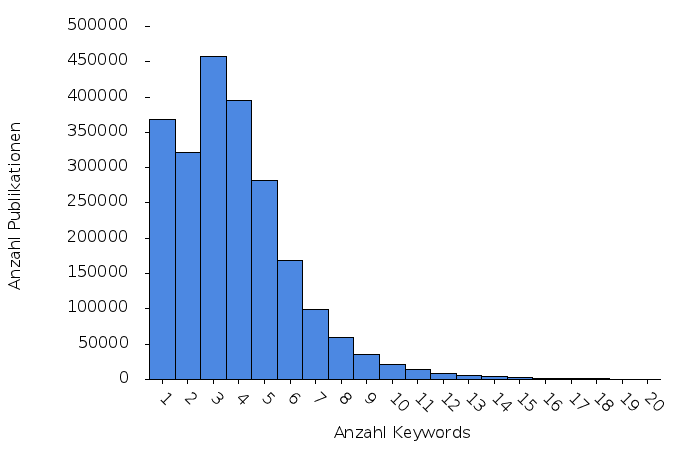
\includegraphics[scale=.5]{../data/statistics/keyWordFreq.png}
        \caption{Keywordverteilung}
        \label{fig:keywordFreqBig}
\end{figure}

\begin{figure}[H]
        \centering
        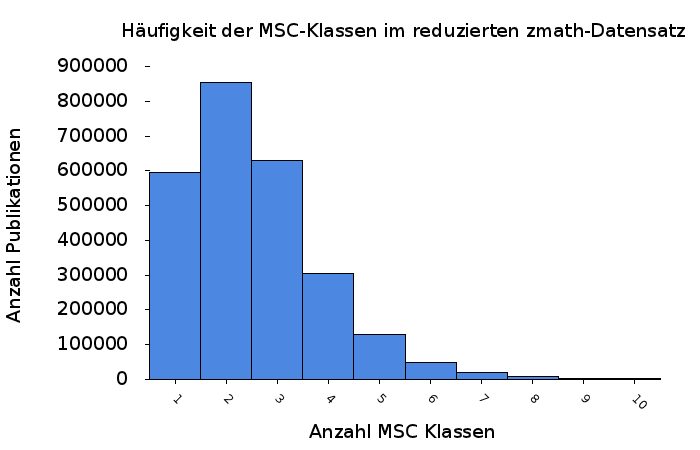
\includegraphics[scale=.5]{../data/statistics/mscClassFreq.png}
        \caption{Verteilung der MSC-Klassen}
        \label{fig:mscClassFreqBig}
\end{figure}

%Kapitel 4
\begin{figure}[H]
        \centering
        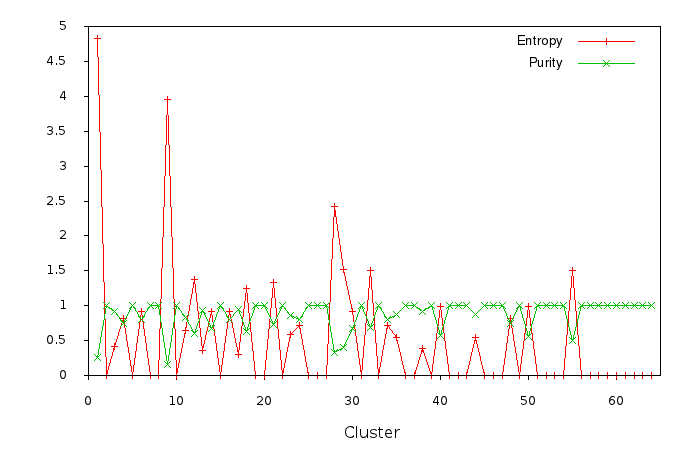
\includegraphics[scale=0.5]{../evaluation/diss_true/crankPurityEntropy.png}
        \caption{Purity und Entropy des \textit{pam}-Clustering von \textit{C-Rank}}
        \label{fig:crankEntPurBig}
\end{figure}


\begin{figure}[H]
        \centering
        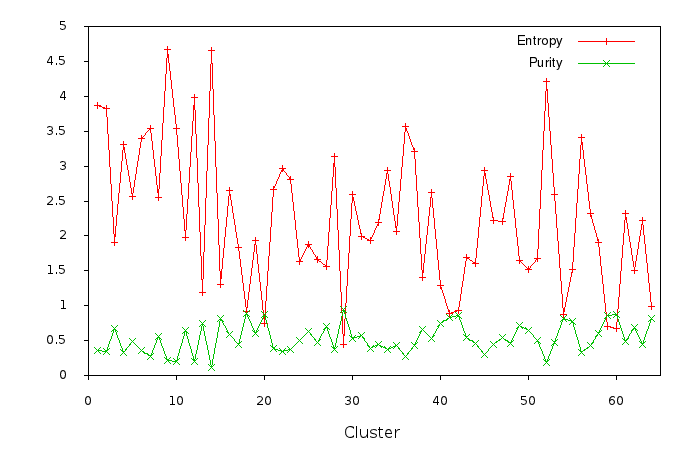
\includegraphics[scale=0.5]{../evaluation/diss_true/p1PurityEntropy.png}
        \caption{Purity und Entropy des \textit{pam}-Clustering von Gewichtung 1}
        \label{fig:p1EntPurBig}
\end{figure}

\begin{figure}[H]
        \centering
        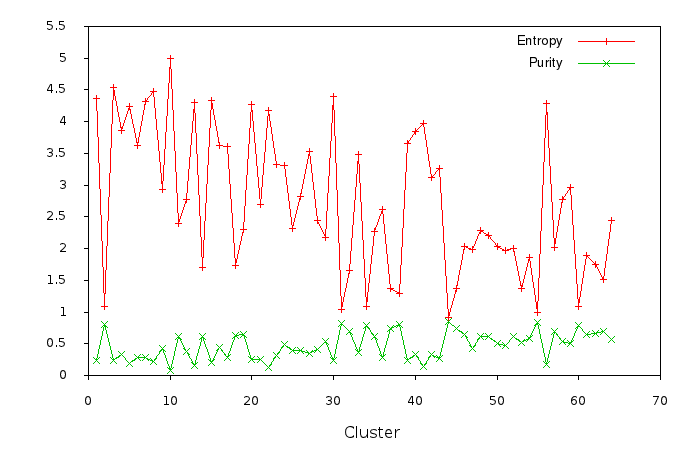
\includegraphics[scale=0.5]{../evaluation/diss_true/p2PurityEntropy.png}
        \caption{Purity und Entropy des \textit{pam}-Clustering von Gewichtung 2}
        \label{fig:p2EntPurBig}
\end{figure}

\begin{figure}[H]
        \centering
        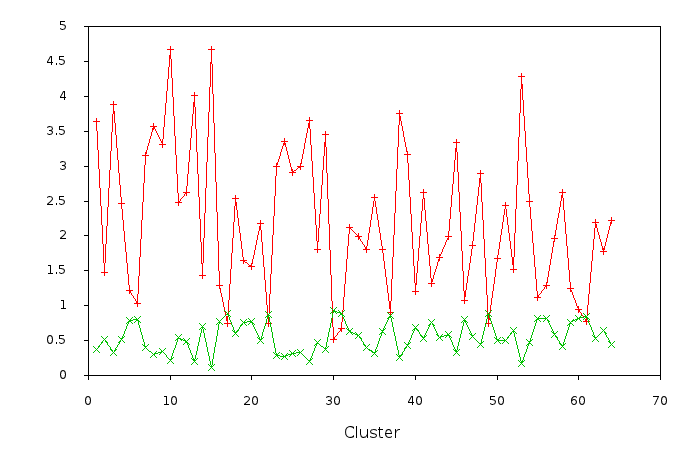
\includegraphics[scale=0.5]{../evaluation/diss_true/p3PurityEntropy.png}
        \caption{Purity und Entropy des \textit{pam}-Clustering von Gewichtung 3}
        \label{fig:p3EntPurBig}
\end{figure}



\subsection*{Berechnung des �hnlichkeitsma�es}
In diesem Appendix wird die erste Iteration, die f�r die Berechnung der semantischen �hnlichkeit erfoderlich ist, f�r zwei Publikationen aus dem \textit{zmath}-Datensatz beispielhaft durchgef�hrt.

\begin{table}[H]
\begin{tabular}{l l}
		%\hline
		\multicolumn{2}{l}{\textbf{Publikation 1}} \\
		%\hline
	    :id: & 3006698 \\
        :an: & 0005.25102\\
        :py: & 1931\\
        :au: & Myrberg, P.J.\\
        :ai: & myrberg.pekka-j\\
        :ti: & �ber beschr�nkte Funktionen in mehrfach zusammenh�ngenden Bereichen.\\
        :so: & Ann. Acad. Sci. Fenn., Ser. A 33, No.8, 1-15 (1931).\\
        :ut: & complex functions\\
        :la: & DE \\
	    %\hline
\end{tabular}
\end{table}

\begin{table}[H]
\begin{tabular}{l p{10cm}}
		%\hline
	    \multicolumn{2}{l}{\textbf{Publikation 2}} \\
		%\hline
	    :id: & 5166522\\
        :an: & 1153.00002\\
        :py: & 2005\\
        :au: & Leonov, Sergey A.; Leonov, Alexander I.\\
        :ai: & leonov.sergey-a; leonov.alexander-i\\
        :ti: & Mathematical handbook for electrical engineers.\\
        :so: & Artech House Technology Management and Professional Development Library. London: Artech House (ISBN 978-1-58053-779-7/hbk). xviii, 495~p. (2005).\\
        :ut: & algebra; functions; equations; combinations; planar and solid geometry; trigonometry; analytic geometry; integral and differential calculus; differential equations; complex functions; Fourier series; vector algebra; probability; applied statistics; computer-aided computation; electrical circuits; antennas; waves; scattering; signal processing; stochastic radio engineering\\
        :la: & EN \\
	    %\hline
\end{tabular}
\end{table}


%::::
%:::
%:id:    5166522
%:an:    1153.00002
%:py:    2005
%:au:    Leonov, Sergey A.; Leonov, Alexander I.
%:ai:    leonov.sergey-a; leonov.alexander-i
%:ti:    Mathematical handbook for electrical engineers.
%:so:    Artech House Technology Management and Professional Development Library. London: Artech House (ISBN 978-1-58053-779-7/hbk). xviii, 495~p. \sterling~85.00 (2005).
%:cc:    00A06 26-00 35-00 60-00 62-00 78-00 94-00
%:ut:    algebra; functions; equations; combinations; planar and solid geometry; trigonometry; analytic geometry; integral and differential calculus; differential equations; complex functions; Fourier series; vector algebra; probability; applied statistics; computer-aided computation; electrical circuits; antennas; waves; scattering; signal processing; stochastic radio engineering
%:la:    EN
%:ci:    
%:li:    


\begin{math}
\begin{array}{lcl}
R_1(P1,P2) & = & 
        \lambda_1\times\cfrac{c}{|K(P1)||K(P2)|}
        \sum_{i=1}^{|K(P1)|} \sum_{j=1}^{|K(P2)|} R_0(K_i(P1),K_j(P2))
        \\ & + &
        \lambda_2\times\cfrac{c}{|A(P1)||A(P2)|}
        \sum_{i=1}^{|A(P1)|} \sum_{j=1}^{|A(P2)|} R_0(A_i(P1),A_j(P2))
        \\ & + &
        \lambda_3\times\cfrac{c}{|S(P1)||S(P2)|}
        \sum_{i=1}^{|S(P1)|} \sum_{j=1}^{|S(P2)|} R_0(S_i(P1),S_j(P2))
        \\ & + &
        \lambda_4\times\cfrac{c}{|C(P1)||C(P2)|}
        \sum_{i=1}^{|C(P1)|} \sum_{j=1}^{|C(P2)|} R_0(C_i(P1),C_j(P2))
        \\ & + &
        \lambda_5\times\cfrac{c}{|Y(P1)||Y(P2)|}
        \sum_{i=1}^{|Y(P1)|} \sum_{j=1}^{|Y(P2)|} R_0(Y_i(P1),Y_j(P2))
        \\ & &
        \\ & = &
        \lambda_1 * \cfrac{c}{1*21} * (R_0(K_1(P1),K_1(P2)) + R_0(K_1(P1),K_2(P2))+
        \\ & &
        \\ & & ... + R_0(K_1(P1),K_{21}(P2)))
        \\ & + &
        \lambda_2 * \cfrac{c}{1*2} * (R_0(A_1(P1),A_1(P2)) + R_0(A_1(P1),A_2(P2)))
        \\ & + &
        \lambda_3 * \cfrac{c}{1*1} * R_0(S_1(P1),S_1(P2))
        \\ & + &
        0
        \\ & + &
        \lambda_5 * \cfrac{c}{1*1} * R_0(Y_1(P1),Y_1(P2))
        \\ & = &
        \lambda_1 * \cfrac{c}{1*21}*(0 + 0 +... +0 + 1 + 0 + ..+ 0)
        \\ & + &
        \lambda_2 * \cfrac{c}{1*2} * (0 + 0)
        \\ & + &
        \lambda_3 * \cfrac{c}{1*1} * 0
        \\ & + &
        0
        \\ & + &
        \lambda_5 * \cfrac{c}{1*1} * 0
        \\ & = &
        \lambda_1 * \cfrac{c}{21} * 1


\end{array}
\end{math}

\bigskip
Dieser erste Iterationsschritt wird auch f�r alle Kombinationen aus jeweils zwei Keywords, zwei Autoren, zwei Quellen und zwei Erscheinungsjahre ausgef�hrt.
F�r jedes Paare derselben Klasse (z.B. zwei Keywords) wird die �hnlichkeit nach der folgenden Formel bestimmt.
Dabei sind L(a) die Publikationen, die das Keyword $a$ verwenden.
Es kann hier leider kein wahrheitsgetreuer Iterationsschritt f�r Keywords beispielhaft vorgef�hrt werden, da wir daf�r alle Publikationen im Datensatz, die diese Keywords verwenden, raussuchen sollten.
Ein Anfang der �hnlichkeitsberechnung f�r die Keywords \textit{complex functions} und \textit{Fourier series} wird folgenderma�en aussehen.
\medskip

\begin{math}
\begin{array}{lcl}
R_1(a,b) &  = &
        \cfrac{c}{|L(a)||L(b)|} *
        \sum_{i=1}^{|L(a)|} \sum_{j=1}^{|L(b)|} R_0(L_i(a),L_j(b))
        \\ & = &
        \cfrac{c}{|L(a)||L(b)|} * (R_0(L_1(a), L_1(b)) + R_0(L_1(a),L_2(b)) + ... + R_0(L_n(a),L_m(b)))
        \\ & = &
        \cfrac{c}{|L(a)||L(b)|} * (... + R_0(P2,P2) + ..)
        \\ & = &
        \cfrac{c}{|L(a)||L(b)|} * (... + 1 + ..)

\end{array}
\end{math}


\bigskip
Bei dem zweiten Iterationsschritt werden dann die Werte aus dem Ersten eingesetzt.
$R_2$ wird aufgrund von $R_1$ berechnet.
